\begin{table*}
  % \vspace{-0.7cm}
\small
\centering

\begin{tabular}{L{3.6cm} L{1.9cm}| r |r| r |r}
\hline

\hline

\hline
Backbone  & Decoder & Params  &FLOPs & mIoU & Latency\\
\hline

\hline
\hline
MobileNetV2 &  LR-ASPP &  2.2M & 2.8G & 32.0 & 177ms \\
MobileNetV3-Lr &  LR-ASPP &  1.6M & 1.3G & 32.3 & 81ms \\
MobileNetV3-Large &  LR-ASPP &  3.2M & 2.0G & 33.1 & 126ms \\
HRNet-W18-Small  &  HRNetW18S  &  4.0M  & 10.2G  & 33.4  & 639ms \\
TopFormer-T &  Simple Head &  1.4M  & 0.6G  & 33.6  & 43ms   \\
TopFormer-T* &  Simple Head &  1.4M  & 0.6G  & 34.6  & 43ms   \\
\textbf{SeaFormerT}  &  Light Head &  1.7M    & 0.6G   & 35.0      & 40ms\\
\textbf{SeaFormer-T*}  &  Light Head &  1.7M    & 0.6G  & 35.8 & 40ms\\
\textbf{SeaFormer-T++}  &  Light Head &  1.8M    & 0.6G  & \textbf{36.8} & 41ms\\
\textbf{SeaFormer-T++(KD)}  &  Light Head &  2.3M    & 0.3G  & 35.5 & \textbf{22ms}\\
\hline

\hline
\hline
ConvMLP-S &  SemanticFPN &  12.8M & 33.8G & 35.8 & 777ms \\
EfficientNet &  DeepLabV3+  &17.1M & 26.9G & 36.2 & 970ms \\
MobileNetV2 &  Lite-ASPP  & 2.9M & 4.4G & 36.6 & 235ms \\
TopFormer-S  &  Simple Head &  3.1M   & 1.2G   & 36.5  & 74ms   \\
TopFormer-S*  &  Simple Head &  3.1M   & 1.2G   & 37.0  & 74ms   \\
\textbf{SeaFormer-S}  &  Light Head &  4.0M     & 1.1G   & 38.1   & 67ms\\
\textbf{SeaFormer-S*}  &  Light Head &  4.0M    & 1.1G    & 39.4  & 67ms\\
\textbf{SeaFormer-S++}  &  Light Head &  4.1M    & 1.1G    & \textbf{39.7}  & 68ms\\
\textbf{SeaFormer-S++(KD)}  &  Light Head &  5.0M    & 0.5G  & 38.4 & \textbf{33ms}\\
\hline

\hline
\hline
MiT-B0 &  SegFormer &  3.8M & 8.4G & 37.4 & 770ms \\
ResNet18 &  Lite-ASPP  &  12.5M & 19.2G & 37.5 & 648ms \\
ShuffleNetV2-1.5x &  DeepLabV3+ & 16.9M & 15.3G & 37.6 & 960ms\\
MobileNetV2 & DeepLabV3+ & 15.4M  & 25.8G & 38.1 & 1035ms \\
TopFormer-B  &  Simple Head &  5.1M & 1.8G  & 38.3   & 110ms   \\
TopFormer-B*  &  Simple Head &  5.1M & 1.8G  & 39.2   & 110ms   \\
\textbf{SeaFormer-B}  &  Light Head &  8.6M & 1.8G  & 40.2      & 106ms\\
\textbf{SeaFormer-B*}  &  Light Head &  8.6M & 1.8G  & 41.0     & 106ms\\
\textbf{SeaFormer-B++}  &  Light Head &  8.7M & 1.8G  & \textbf{41.4}      & 107ms\\
\textbf{SeaFormer-B++(KD)}  &  Light Head &  10.2M    & 0.9G  & 39.5 & \textbf{55ms}\\
\hline

\hline
\hline
MiT-B1  &  SegFormer &  13.7M & 15.9G  & 41.6   & 1300ms   \\
\textbf{SeaFormer-L}  &  Light Head &  14.0M & 6.5G  & 42.7      & 367ms\\
\textbf{SeaFormer-L*}  &  Light Head &  14.0M & 6.5G  & 43.7      & 367ms\\
\textbf{SeaFormer-L++}  &  Light Head &  14.1M & 6.5G  & \textbf{43.8}      & 369ms\\
\textbf{SeaFormer-L++(KD)}  &  Light Head &  17.1M    & 2.9G  & 42.2 & \textbf{177ms}\\
% \Xhline{5\arrayrulewidth}
\hline

\hline

\hline
\end{tabular}
\caption{Results of semantic segmentation on ADE20K \textit{val} set, * indicates training batch size is 32. KD means knowledge distillation.
The latency is measured on a single Qualcomm Snapdragon 865 with input size 512×512, and only an ARM CPU core is used for speed testing. MobileNetV3-Lr means MobileNetV3-Large-reduce. HRNet-W18S means HRNet-W18-Small.
References:
MobileNetV2~\cite{sandler2018mobilenetv2}, 
MobileNetV3~\cite{howard2019searching},
HRNet~\cite{yuan2020object},
TopFormer~\cite{zhang2022topformer},
ConvMLP~\cite{li2021convmlp},
Semantic FPN~\cite{kirillov2019panoptic},
EfficientNet~\cite{tan2019efficientnet},
DeepLabV3+ and Lite-ASPP~\cite{chen2018encoder},
SegFormer~\cite{xie2021segformer},
ResNet~\cite{he2016deep},
ShuffleNetV2-1.5x~\cite{ma2018shufflenet}.
}
\label{ade20k_table}
% \vspace{-0.2cm}
\end{table*}
\begin{table*}[tb]
% \vspace{-0.5cm}
    \centering
  
    \begin{tabular}[b]{L{2.5cm}  L{2.7cm} |R{1.1cm} C{1.3cm} C{1.3cm} R{1.4cm}}
    \hline

    \hline
    
    \hline
    Method     & Backbone     & FLOPs        & mIoU(val) & mIoU(test)  & Latency\\
    \hline

    \hline
    \hline
    FCN & MobileNetV2 & 317G & 61.5 & - &  24190ms\\
    PSPNet  &   MobileNetV2  & 423G & 70.2 & - & 31440ms\\
    SegFormer(h) & MiT-B0 & 17.7G & 71.9 & - & 1586ms\\
    SegFormer(f) & MiT-B0 & 125.5G & 76.2 & - & 11030ms\\
    L-ASPP & MobileNetV2       & 12.6G & 72.7  & - & 887ms \\
    LR-ASPP & MobileNetV3-L      & 9.7G & 72.4  & 72.6 & 660ms  \\
    LR-ASPP & MobileNetV3-S      & 2.9G & 68.4 & 69.4 & 211ms  \\
    SimpleHead(h) & TopFormer-B       &     2.7G      & 70.7   & - & 173ms    \\
    SimpleHead(f) & TopFormer-B       &     11.2G      & 75.0  & 75.0 & 749ms     \\
    \hline

    \hline
    \hline
    Light Head(h) & \textbf{SeaFormerS}       &   2.0G    & 70.7  & 71.0 & 129ms       \\
    Light Head(h) & \textbf{SeaFormerS++}       &   2.0G    & 72.1  & 72.3 & 130ms       \\
    Light Head(f) & \textbf{SeaFormerS}       &   8.0G    & 76.1  & 75.9 & 518ms        \\
    Light Head(f) & \textbf{SeaFormerS++}       &   8.0G    & 77.2  & 76.9 & 521ms       \\
    Light Head(h) & \textbf{SeaFormerB}       &   3.4G    & 72.2  & 72.5 & 205ms        \\
    Light Head(h) & \textbf{SeaFormerB++}       &   3.4G    & 73.5  & 73.4 & 207ms       \\
    Light Head(f) & \textbf{SeaFormerB}       &   13.7G    & 77.7 & 77.5 & 821ms         \\  
    Light Head(f) & \textbf{SeaFormerB++}       &   13.7G    & 78.6  & 78.3 & 825ms       \\
    \hline

    \hline
    
    \hline
  \end{tabular}
\caption{Results on Cityscapes \textit{val} and \textit{test} set. The results on \textit{test} set of some methods are not presented due to the fact that they are not reported in their original papers.}
\label{table_city}
% \vspace{-0.2cm}
\end{table*}
\section{Experiments}
\label{Exp}
We evaluate our method on semantic segmentation, image classification and object detection tasks.
First, we describe implementation details and compare results with state of the art.
We then conduct a series of ablation studies to validate the design of SeaFormer.
Each proposed component and important hyper-parameters are examined thoroughly.

\subsection{Experimental setup}
\label{sec:experimental_setup}
\subsubsection{Dataset} We perform semantic segmentation experiments over ADE20K~\cite{zhou2017scene}, CityScapes~\cite{cordts2016cityscapes}, Pascal Context~\cite{mottaghi2014role} and COCO-Stuff~\cite{caesar2018coco}.
The mean of intersection over union (mIoU) is set as the evaluation metric. 
We convert full-precision models to TNN~\cite{contributors2020tnn} and measure latency on an ARM-based device with a single Qualcomm Snapdragon 865 processor.

\paragraph{ADE20K} ADE20K dataset covers 150 categories, containing 25K images that are split into 20K/2K/3K for \textit{Train}, \textit{val} and \textit{test}.

\paragraph{CityScapes} CityScapes is a driving dataset for semantic segmentation. It consists of 5000 fine annotated high-resolution images with 19 categories.

\paragraph{PASCAL Context} dataset has 4998 scene images for training and 5105 images for testing. There are 59 semantic labels and 1 background label.

\paragraph{COCO-Stuff} dataset augments COCO dataset with pixel-level stuff annotations. There are 10000 complex images selected from COCO. The training set and test set consist of 9K and 1K images respectively.

\subsubsection{Implementation details}
We set ImageNet-1K~\cite{deng2009imagenet} pretrained network as the backbone, and training details of ImageNet-1K are illustrated in the last subsection. 
For semantic segmentation, the standard BatchNorm~\cite{ioffe2015batch} layer is replaced by synchronized BatchNorm.
Our implementation is based on public codebase \texttt{mmsegmentation}~\cite{contributors2020mmsegmentation}.
We follow the batch size, training iteration scheduler and data augmentation strategy of TopFormer~\cite{zhang2022topformer} for a fair comparison.

\paragraph{ADE20K} The initial learning rate is 0.0005 for batch size 32 or 0.00025 for batch size 16. The weight decay is 0.01. 
A “poly” learning rate scheduled with factor 1.0 is adopted.

\paragraph{Cityscapes} The initial learning rate is 0.0003 and the weight decay is 0.01.
The comparison of Cityscapes contains full-resolution and half-resolution.
For the full-resolution version, the training images are randomly scaled and then cropped to the fixed size of 1024 × 1024. 
For the half-resolution version, the training images are resized to 1024 × 512 and randomly scaling, the crop size is 1024 × 512. 

\paragraph{Pascal Context} The initial learning rate is 0.0002 and the weight decay is 0.01. A poly learning rare scheduled with factor 1.0 is used. 

\paragraph{COCO-Stuff} The initial learning rate is 0.0002 and the weight decay is 0.01. A poly learning rare scheduled with factor 1.0 is used. 

During inference, we set the same resize and crop rules as TopFormer to ensure fairness.

\subsection{Comparison with state of the art}

\paragraph{ADE20K}
Table~\ref{ade20k_table} shows the results of SeaFormer and previous efficient backbones on ADE20K \textit{val} set. 
The comparison covers Params, FLOPs, Latency and mIoU. 
As shown in Table~\ref{ade20k_table}, SeaFormer outperforms these efficient approaches with comparable or less FLOPs and lower latency. 
Compared with specially designed mobile backbone, TopFormer, which sets global self-attention as its semantics extractor, SeaFormer achieves higher segmentation accuracy with lower latency. 
And the performance of SeaFormer-B++ surpasses MobileNetV3 by a large margin of +8.3\% mIoU with lower latency (-16\%). The results demonstrate that our SeaFormer layers improve the representation capability significantly.



\paragraph{Cityscapes}
From the table~\ref{table_city}, it can be seen that SeaFormer-B++ is 1.3 points better than SeaFormer-B with only a slight increase in latency, showing the benefit of our efficient architecture design with multiple SeaFormer layers embedded in.
It is worth noting that with less computation cost and latency, our SeaFormer-S and SeaFormer-S++ even outperform TopFormer-B. This result further confirms the performance and efficiency of our model when processing high-resolution input images.

\paragraph{Pascal Context}
We compare SeaFormer with the previous approaches on Pascal Context validation set in Table~\ref{pascal_table}. We evaluate the performance over 59 categories and 60 categories (including background). From the results, it can be seen that SeaFormer-S++ is +1.2\% mIoU higher (46.31\% vs.45.08\%) than SeaFormer-S with similar latency. 

\paragraph{COCO-Stuff}
We compare SeaFormer with the previous approaches on COCO-Stuff validation set in Table~\ref{coco-stuff_table}. From the results, it can be seen that SeaFormer-S++ is +1.2\% mIoU higher (34.04 \vs 32.82) than SeaFormer-S with similar computation cost.
\begin{table}
% \small
\centering
    \begin{tabular}{ll |c | c}
        \hline

        \hline

        \hline
    Backbone     & Decoder     & FLOPs     &mIoU (60/59) \\
        \hline

        \hline
        \hline
    MBV2-s16 &  DeepLabV3+  &  22.24G &  38.59/42.34 \\
    ENet-s16 & DeepLabV3+  & 23.00G & 39.19/43.07 \\
        \hline

        \hline
        \hline
    MBV3-s16 &  LR-ASPP &  2.04G & 35.05/38.02 \\
    TopFormer-T  &  Simple Head &  0.53G  & 36.41/40.39   \\
    SeaFormer-T  &  Light Head &  0.51G   & 37.27/41.49  \\
    \textbf{SeaFormer-T++}  &  Light Head &  0.52G   & \textbf{38.61}/\textbf{42.56}  \\
        \hline

        \hline
        \hline    
    TopFormer-S &  Simple Head &  0.98G   & 39.06/43.68   \\
    SeaFormer-S  & Light Head &  0.98G  & 40.20/45.08   \\
    \textbf{SeaFormer-S++}  & Light Head &  1.00G  & \textbf{41.44}/\textbf{46.31}   \\
        \hline

        \hline
        \hline   
    TopFormer-B & Simple Head &  1.54G   & 41.01/45.28   \\
    SeaFormer-B   & Light Head & 1.57G    & 41.77/45.92   \\
    \textbf{SeaFormer-B++}   & Light Head & 1.60G    & \textbf{42.52}/\textbf{46.40}   \\
        \hline

        \hline

        \hline
  \end{tabular}
\caption{Results on Pascal Context \textit{val} set. We omit the latency as the input resolution is almost the same as that in table 1.}
\label{pascal_table}

\end{table}
\begin{table}
\vspace{-0cm}
% \small
\centering
    \begin{tabular}{ll |c | c}
        \hline

        \hline
        
        \hline
    Backbone  &  Decoder  & FLOPs     & mIoU  \\
        \hline

        \hline
        \hline
    MBV2-s8 & PSPNet& 52.94G & 30.14  \\
    ENet-s16& DeepLabV3+  & 27.10G & 31.45\\
        \hline

        \hline
        \hline
    MBV3-s16 & LR-ASPP & 2.37G &  25.16 \\
    TopFormer-T  & Simple Head & 0.64G & 28.34   \\
    SeaFormer-T & Light Head & 0.62G & 29.24   \\
   \textbf{ SeaFormer-T++} & Light Head & 0.63 & \textbf{30.76}   \\
        \hline

        \hline
        \hline  
    TopFormer-S  & Simple Head & 1.18G & 30.83  \\
    SeaFormer-S  & Light Head & 1.15G  & 32.82    \\
    \textbf{SeaFormer-S++}  & Light Head & 1.17G  & \textbf{34.04}    \\
        \hline

        \hline
        \hline    
    TopFormer-B  & Simple Head & 1.83G & 33.43\\
    SeaFormer-B  & Light Head &  1.81G  & 34.07 \\
    \textbf{SeaFormer-B++}  & Light Head &  1.84G  & \textbf{35.01} \\
        \hline

        \hline
        
        \hline
  \end{tabular}
\caption{Results on COCO-Stuff \textit{test} set. We omit the latency in this table as the input resolution is the same as that in table 1.}
\label{coco-stuff_table}

\end{table}


\subsection{Ablation studies}
In this section, we ablate different self-attention implementations and some important design elements in the proposed model, including our squeeze-enhanced Axial attention module (SEA attention) and fusion block on ADE20K dataset.

\paragraph{The influence of components in SEA attention}
We conduct experiments with several configurations, including detail enhancement kernel only, squeeze Axial attention only, and the fusion of both. 
As is shown in Table~\ref{ablate_attn}, only detail enhancement or squeeze Axial attention achieves a relatively poor performance, and enhancing squeeze Axial attention with detail enhancement kernel brings a performance boost with a gain of 2.3\% mIoU on ADE20K. 
The results indicate that enhancing global semantic features from squeeze Axial attention with local details from convolution optimizes the feature extraction capability of Transformer block. 
For enhancement input, there is an apparent performance gap between upconv(x) and conv(x). And we conclude that increasing the channels will boost performance significantly.
Comparing concat[qkv] and upconv(x), which also correspond to w/ or w/o convolution weight sharing between detail enhancement kernel and squeeze Axial attention, we can find that sharing weights makes our model improve inference efficiency with minimal performance loss (35.8 \vs 35.9).
As for enhancement modes, multiplying features from squeeze Axial attention and detail enhancement kernel outperforms add enhancement by +0.4\% mIoU. 
\begin{table*}[htb]
% \vspace{-0.5cm}
  \centering


      \begin{tabular}{C{1.0cm} C{1.0cm} |C{1.6cm} C{1.2cm} | C{0.9cm} C{0.8cm}  C{1.0cm} C{0.6cm}  C{0.6cm}}
        \hline

        \hline

        \hline
        Enhance  & Attn & Enhance & Enhance  & \multirow{2}{*}{Params}     & \multirow{2}{*}{FLOPs}    & \multirow{2}{*}{Latency}     & \multirow{2}{*}{Top1}     &  \multirow{2}{*}{mIoU} \\
        kernel      &  branch   & input &  mode   &        &        &         &     &   \\
        \hline

        \hline
        \hline
        \ding{52}  &  & - &  -  &  1.3M  & 0.58G  & 38ms &  65.9  & 32.5 \\
          &   \ding{52} & - &  -   & 1.4M & 0.57G & 38ms & 66.3 & 33.5 \\
        \ding{52} & \ding{52} & conv(x) & Mul  & 1.6M     & 0.60G     & 40ms    & 67.2   & 34.9   \\
        \ding{52} & \ding{52} & upconv(x) & Mul  & 1.8M     & 0.62G     & 41ms    & 68.1   & 35.9   \\
        \ding{52} & \ding{52} & concat[qkv] & Mul  & 1.7M     & 0.60G     & 40ms    & 67.9   & 35.8   \\
        \ding{52} & \ding{52} & concat[qkv] & Add  & 1.7M     & 0.60G     & 40ms    & 67.3   & 35.4   \\
        \hline

        \hline

        \hline
    \end{tabular}
    \caption{Ablation studies on components in SEA attention on ImageNet-1K and ADE20K datasets. Enhancement input means the input of detail enhancement kernel. conv(x) means x followed by a point-wise conv. upconv(x) is the same as conv(x) except different channels as upconv(x) is from  $C_{in}$ to $C_q+C_k+C_v$ and conv(x) is from $C_{in}$ to $C_{in}$. concat[qkv] indicates concatenation of Q,K,V.}
    \label{ablate_attn}
% \vspace{-0.2cm}
\end{table*}
\begin{table*}[htb]
% \vspace{-0.5cm}
  \centering


      \begin{tabular}{c c  | c c c c c}
        \hline

        \hline

        \hline
        Squeeze method  & Expand method   & {Params}     & {FLOPs}    & {Latency}     & {Top1}     &  {mIoU} \\
        \hline

        \hline
        \hline
        Mean pooling & Broadcast  & 1.7M     & 0.60G    & 40ms    & 67.9  & 35.8   \\
        Max pooling & Broadcast  & 1.7M     & 0.60G     & 40ms    & 67.4   & 35.0   \\
        Adaptive squeeze & Adaptive expand & 1.8M     & 0.61G     & 41ms    & 69.8   & 36.8   \\
        \hline

        \hline

        \hline
    \end{tabular}
    \caption{Ablation studies on squeeze and expand methods in SEA attention on ImageNet-1K and ADE20K datasets.}
    \label{ablate_adasqueeze}
% \vspace{-0.2cm}
\end{table*}

\paragraph{Comparison with different self-attention modules}
\begin{table}
    % \vspace{-0.4cm}
    \centering
    \small
 
    \begin{tabular}[b]{l | c |c |c | c}

    \hline
    Model     & Params(B)     & FLOPs(B)        & mIoU  & Latency\\
    \hline

    Swin	&27.5M	&25.6G	&44.5	&3182ms\\
    CCNet	&41.6M	&37.4G	&43.1	&3460ms\\
    ISSA	&31.8M	&33.3G	&37.4	&2991ms\\
    A2-Nets	&37.2M	&31.1G	&28.9	&2502ms\\
    Axial	&36.2M	&32.5G	&45.3	&3121ms\\
    Local	&27.5M	&25.1G	&34.2	&3059ms\\
    MixFormer	&27.5M	&24.9G	&45.5	&2817ms\\
    ACmix	&27.9M	&26.6G	&45.3	&3712ms\\
    Global	&27.5M	&0.144T	&OOM	&14642ms\\

    \hline

    \textbf{SeaFormer}	&34.0M	&\textbf{24.9G}	&\textbf{46.5} &\textbf{2278ms}\\

    \hline
  \end{tabular}
\caption{Results on ADE20K \textit{val} set based on Swin Transformer architecture. (B) denotes backbone. OOM means CUDA out of memory. References: ISSA~\cite{huang2019interlaced}, A2-Nets~\cite{chen20182}}
\label{table_swin} 
% \vspace{-0.4cm}
\end{table}
To eliminate the impact of our architecture and demonstrate the effectiveness and generalization ability of SEA attention, we ran experiments on Swin Transformer~\cite{liu2021swin} by replacing window attention in Swin Transformer with different attention blocks.
We set the same training protocol, hyper-parameters, and model architecture configurations as Swin for a fair comparison. 
When replacing window attention with CCAttention (CCNet) or DoubleAttention (A2-Nets), they have much lower FLOPs than SeaFormer and other attention blocks. 
Considering that we may not be able to draw conclusions rigorously, we doubled the number of their Transformer blocks (including MLP).
As ACmix has the same architecture configuration as Swin, we borrow the results from the original paper. 
From Table~\ref{table_swin}, it can be seen that SeaFormer outperforms other attention mechanisms with lower FLOPs and latency.

\paragraph{Effective and efficiency of SEA attention}
To verify the effectiveness and efficiency of SEA attention based on our designed pipeline, we experiment with convolution, Global attention, Local attention, Axial attention and three convolution enhanced attention methods including our SEA attention, ACmix and MixFormer. 
The ablation experiments are organized in seven groups.
Since the resolution of computing attention is relatively small, the window size in Local attention, ACmix, and MixFormer is set to 4.
We adjust the channels when applying different attention modules to keep the FLOPs aligned and compare their performance and latency.
The results are illustrated in Table~\ref{table_attn}.

As demonstrated in the table, SEA attention outperforms the counterpart built on other efficient attentions.
Compared with global attention, SEA attention outperforms it by +1.2\% Top1 accuracy on ImageNet-1K and +1.6 mIoU on ADE20K with less FLOPs and lower latency. 
Compared with similar convolution enhanced attention works, ACmix and MixFormer, our SEA attention obtains better results on ImageNet-1K and ADE20K with similar FLOPs but lower latency. 
The results indicate the effectiveness and efficiency of SEA attention module.
\begin{table}

    \centering
    \small


        % \begin{tabular}{L{1.5cm}| C{0.6cm} |C{0.6cm} | C{0.6cm} | C{0.6cm} |C{0.6cm}}
        \begin{tabular}{l | c | c| c| c| c}
        \hline
        
        \hline

        \hline
        Method     & Params   & FLOPs   & Latency     & Top1    &  mIoU  \\
        \hline

        \hline
        \hline
        Conv  &  1.6M  & 0.59G  & 38ms &  66.3  & 32.8 \\
        Local & 1.3M  &  0.60G  & 48ms &  65.9 & 32.8  \\
        Axial & 1.6M  &  0.63G  & 44ms &  66.9 & 33.7  \\
        Global & 1.3M & 0.61G  & 43ms & 66.7 & 34.2 \\
        ACmix &   1.3M  & 0.60G & 54ms & 66.0 & 33.1 \\
        MixFormer &   1.3M & 0.60G  & 50ms & 66.8 & 33.8 \\
        % Local~\cite{luong2015effective} & 1.4M  &  0.60G  & 41ms &  65.9 & 32.9  \\
        % Axial~\cite{ho2019axial} & 1.5M  &  0.61G  & 41ms &  66.4 & 33.5  \\
        % Global~\cite{vaswani2017attention} & 1.2M & 0.60G  & 41ms & 66.2 & 34.0 \\
        % ACmix~\cite{pan2021integration} &   1.2M  & 0.60G & 54ms & 66.0 & 33.1 \\
        % MixFormer~\cite{chen2022mixformer} &   1.3M & 0.59G  & 48ms & 66.8 & 33.6 \\
        \textbf{SeaFormer} & 1.7M & 0.60G & \textbf{40ms}  & \textbf{67.9}  & \textbf{35.8}  \\
        \hline

        \hline

        \hline
    \end{tabular}
    \caption{Performance of different self-attention modules on our designed pipeline on ImageNet-1K and ADE20K datasets. 
    % \texttt{P} means \texttt{Parameters}, \texttt{F} means \texttt{Flops}, \texttt{L} means latency.
    }
    \label{table_attn}
\vspace{-0.1cm}
\end{table}

\paragraph{The influence of squeeze and expand method}
To evaluate different squeeze and expand strategies within the SEA attention framework, we conducted a structured series of ablation studies. These were divided into three groups based on the method used, focusing on maintaining consistent FLOPs, latency, and comparative performance on the ImageNet-1K and ADE20K datasets.

Table~\ref{ablate_adasqueeze} summarizes the outcomes. Notably, the `Adaptive squeeze and Adaptive expand` method excelled, achieving 69.8\% Top1 accuracy on ImageNet-1K and 36.8 mIoU on ADE20K. This method outperformed the `Mean pooling` and `Max pooling` methods combined with `Broadcast` expansion, both of which showed similar FLOPs and latency but lower performance metrics.

\paragraph{The influence of fusion block design}
We set four fusion methods, including "Add directly", "Multiply directly", "Sigmoid add" and "Sigmoid multiply". \textbf{X} directly means features from context branch and spatial branch \textbf{X} directly. 
Sigmoid \textbf{X} means feature from context branch goes through a sigmoid layer and \textbf{X} feature from spatial branch.

From the Table~\ref{table_fusion} we can see that replacing sigmoid multiply with other fusion methods hurts performance. 
Sigmoid multiply is our optimal fusion block choice.
\begin{table}[tb]
    \centering
        \begin{tabular}{l|c}
        
        \hline
        
        \hline
        
        \hline
        Fusion method  &  mIoU  \\
        \hline
        
        \hline
        \hline
        Add directly&	35.2\\
        Multiply directly&	35.2\\
        Sigmoid add	&34.8\\
        \textbf{Sigmoid multiply}&	\textbf{35.8}\\
        \hline
        
        \hline
        
        \hline
    \end{tabular}
    \caption{Ablation study on fusion method on ADE20K \textit{val} set.}
        \label{table_fusion}
\end{table}
\begin{table}
% \vspace{-0.9cm}
    \centering
    \small

        \begin{tabular}{C{0.9cm} | C{0.8cm} |C{0.8cm} | C{0.9cm} |C{0.6cm}}
        
        \hline


        M  & Params     & FLOPs    & Latency    &  mIoU \\
        \hline

        64,96        & 8.5M          & 1.7G      & 102ms   & 40.3 \\
        128,160       & 8.6M          & 1.8G      & 106ms   &  41.0\\
        192,256       & 8.7M          & 2.0G      & 121ms   &  41.2\\
        \hline


        \end{tabular}
        \vspace{0.14cm} 
        \begin{tabular}{C{0.9cm} | C{0.8cm} |C{0.8cm} | C{0.9cm} |C{0.6cm}}
        \hline


        Posbias   & Params     & FLOPs    & Latency    &  mIoU \\
        \hline

        
            \ding{56} & 1.65M       & 0.60G          & 40ms      & 35.6   \\
            \ding{52} & 1.67M       & 0.60G          & 40ms      & 35.8   \\
        \hline


    \end{tabular}
    \caption{Ablation studies on embedding dimensions and position bias.M = [128, 160] is an optimal embedding dimension in fusion blocks.}
    \label{table_embdim_posbias}
    % \vspace{-0cm}
\end{table}

\paragraph{The influence of the width in fusion block}
To study the influence of the width in fusion block, we perform experiments with different embedding dimensions in fusion blocks on SeaFormer-Base, M denotes the channels that spatial branch and context branch features mapping to in two fusion blocks. Results are shown in Table~\ref{table_embdim_posbias}.

\begin{table}
% \vspace{-1.1cm}
\small
\centering

\begin{tabular}{L{4.0cm}|C{1.5cm}|C{1.5cm}|C{1.5cm}|C{1.5cm}}
\hline

\hline

\hline
Method  & Params  &FLOPs & Top1 & Latency\\
\hline

\hline
\hline
MobileNetV3-Small~\cite{howard2019searching}  & 2.9M & 0.1G & 67.4 & \textbf{5ms} \\
SeaFormer-T  & 1.8M & 0.1G & 67.9 & 7ms \\
\textbf{SeaFormer-T++}  & 1.9M & 0.1G & \textbf{69.8} & 7ms \\
\hline

\hline
\hline
MobileViT-XXS~\cite{mehta2021mobilevit}  & 1.3M & 0.4G & 69.0 & 24ms \\
MobileViTv2-0.50~\cite{mehta2022separable} & 1.4M & 0.5G & 70.2 & 32ms \\
MobileOne-S0*~\cite{vasu2022improved} & 2.1M & 0.3G & 71.4 & 14ms \\
MobileNetV2~\cite{sandler2018mobilenetv2} & 3.4M & 0.3G & 72.0 & 17ms \\
Mobile-Former96~\cite{chen2022mobile} & 4.8M & 0.1G & 72.8 & 31ms \\
SeaFormer-S & 4.1M & 0.2G & 73.3 & 12ms \\
\textbf{SeaFormer-S++} & 4.2M & 0.2G & \textbf{74.5} & \textbf{12ms} \\
\hline

\hline
\hline
EdgeViT-XXS~\cite{pan2022edgevits} & 4.1M & 0.6G & 74.4  & 71ms \\
LVT~\cite{yang2022lite} & 5.5M & 0.9G & 74.8 & 97ms \\
MobileViT-XS~\cite{mehta2021mobilevit} & 2.3M & 0.9G & 74.8 & 54ms \\
MobileNetV3-Large~\cite{howard2019searching} & 5.4M & 0.2G & 75.2 & \textbf{16ms} \\
Mobile-Former151~\cite{chen2022mobile} & 7.7M & 0.2G & 75.2 & 42ms \\
MobileViTv2-0.75~\cite{mehta2022separable} & 2.9M & 1.0G & 75.6 & 68ms \\
MobileOne-S1*~\cite{vasu2022improved} & 4.8M & 0.8G & 75.9 & 40ms \\
SeaFormer-B & 8.7M & 0.3G & 76.0 & 20ms \\
\textbf{SeaFormer-B++} & 8.8M & 0.3G & \textbf{77.0} & 20ms \\
\hline

\hline
\hline
MobileOne-S2*~\cite{vasu2022improved} & 7.8M & 1.3G & 77.4 & 63ms \\
EdgeViT-XS~\cite{pan2022edgevits} & 6.8M & 1.1G & 77.5  & 124ms \\
MobileViTv2-1.00~\cite{mehta2022separable} & 4.9M & 1.8G & 78.1 & 115ms \\
MobileOne-S3*~\cite{vasu2022improved} & 10.1M & 1.9G & 78.1 & 91ms \\
MobileViT-S~\cite{mehta2021mobilevit} & 5.6M & 1.8G & 78.4 & 88ms \\
EfficientNet-B1~\cite{tan2019efficientnet} & 7.8M & 0.7G & 79.1 & 61ms \\
EfficientFormer-L1~\cite{li2022efficientformer} & 12.3M & 1.3G & 79.2 & 94ms \\
Mobile-Former508~\cite{chen2022mobile}  & 14.8M & 0.5G & 79.3 & 102ms \\
MobileOne-S4*~\cite{vasu2022improved} & 14.8M & 3.0G & 79.4 & 143ms \\
SeaFormer-L & 14.0M & 1.2G & 79.9 & 61ms \\ 
\textbf{SeaFormer-L++} & 14.1M & 1.2G & \textbf{80.6} & \textbf{61}ms \\ 
\hline

\hline

\hline
\end{tabular}
\caption{Image classification results on ImageNet-1K \textit{val} set. The FLOPs and latency are measured with input size 224×224, except for MobileViT and MobileViTv2 that are measured with 256×256 according to their original implementations. * indicates re-parameterized variants~\cite{vasu2022improved}. The latency is measured on a single Qualcomm Snapdragon 865, and only an ARM CPU core is used for speed testing. No other means of acceleration, e.g., GPU or quantification, is used.}
\label{imagenet_table}
% \vspace{-2.2cm}
\end{table}
\subsection{Image classification}
\label{sec:imgnet_training}
We conduct experiments on ImageNet-1K~\cite{deng2009imagenet}, which contains 1.28M training images and 50K validation images from 1,000 classes. We employ an AdamW~\cite{kingma2014adam} optimizer for 600 epochs using a cosine decay learning rate scheduler. A batch size of 1024, an initial learning rate of 0.064, and a weight decay of 2e-5 are used. The results are illustrated in Table~\ref{imagenet_table}. Compared with other efficient approaches, SeaFormer++ achieves a relatively better trade-off between latency and accuracy.

\begin{figure*}[tbp]
	\centering
	\subfloat[Squeeze Axial attention heatmaps]{\label{heatmap_vis_saa}
	                                        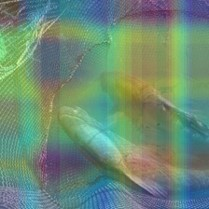
\includegraphics[width=1.2in, height=1.in]{Axial1.jpg}
	                                        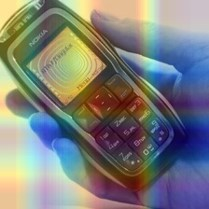
\includegraphics[width=1.2in, height=1.in]{Axial3.jpg}
	                                        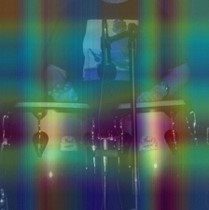
\includegraphics[width=1.2in, height=1.in]{Axial4.jpg}
	                                        
\includegraphics[width=1.2in, height=1.in]{Axial5.jpg}
	                                        }\\
	\subfloat[Squeeze-enhanced Axial attention heatmaps]{\label{heatmap_vis_sea}   
	                                        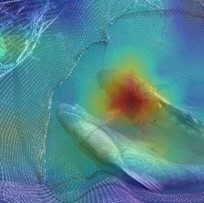
\includegraphics[width=1.2in, height=1.in]{Sea1.jpg}
	                                        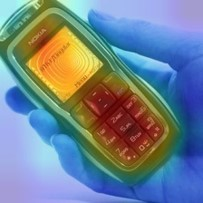
\includegraphics[width=1.2in, height=1.in]{Sea3.jpg}
	                                        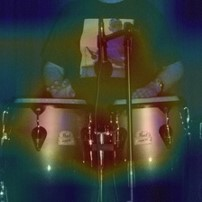
\includegraphics[width=1.2in, height=1.in]{Sea4.jpg}
	                                        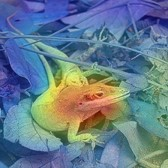
\includegraphics[width=1.2in, height=1.in]{Sea5.jpg}
	                                        }\\	
	\centering
	\caption{The visualization of attention heatmaps from the model consisting of squeeze Axial attention without detail enhancement (\textit{first row}) and SeaFormer (\textit{second row}). Heatmaps are produced by  averaging channels of the features from the last attention block, normalizing to [0, 255] and up-sampling to the image size.}

	\label{heatmap_vis}
\end{figure*}
\begin{figure*}[tbp]
	\centering
	\subfloat[Ground Truth]{
               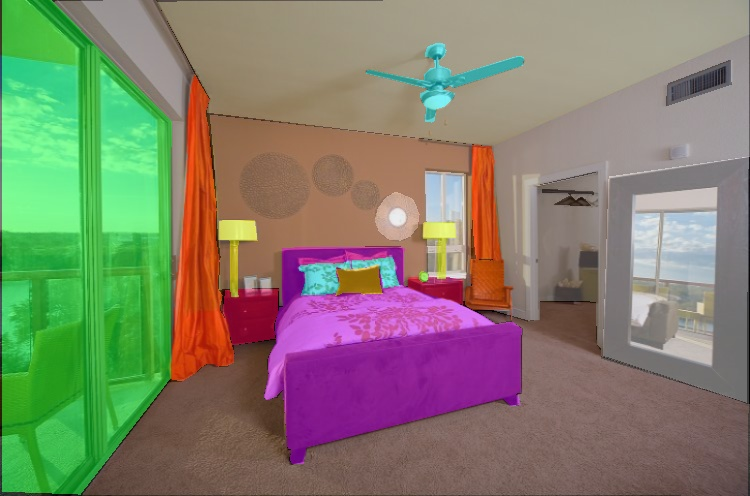
\includegraphics[width=1.5in, height=1.in]{gt_00000129.jpg} 
               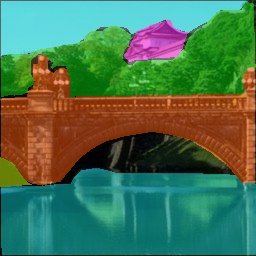
\includegraphics[width=1.5in, height=1.in]{gt_00000200.jpg} 
               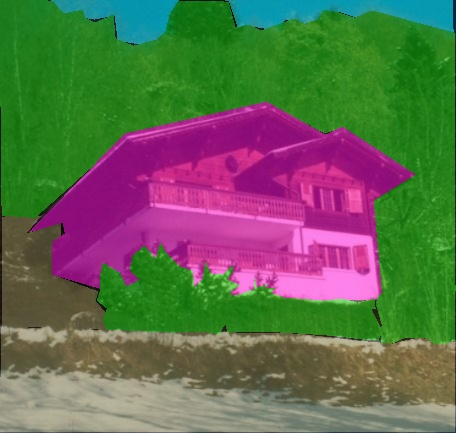
\includegraphics[width=1.5in, height=1.in]{gt_00001239.jpg} 
	                                        }\\
	\subfloat[TopFormer-B~\cite{zhang2022topformer}]{
                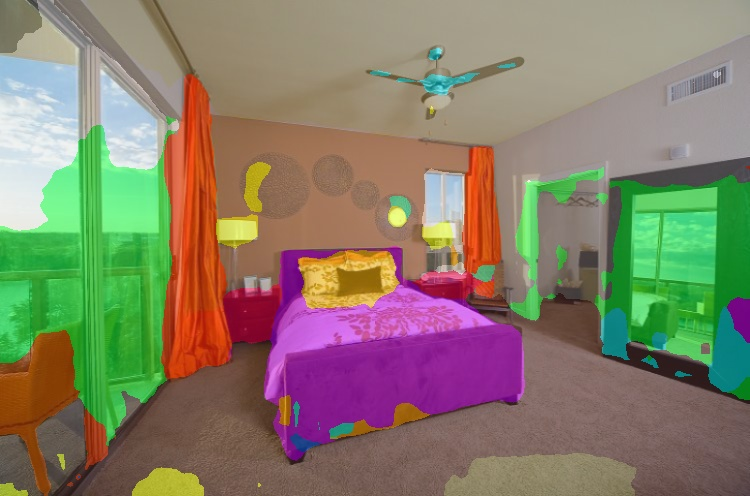
\includegraphics[width=1.5in, height=1.in]{Top_00000129.jpg} 
                
\includegraphics[width=1.5in, height=1.in]{Top_00000200.jpg} 
                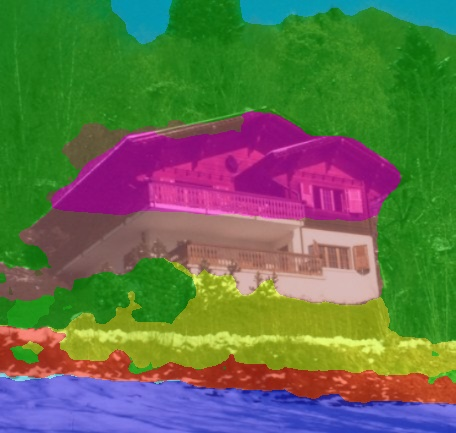
\includegraphics[width=1.5in, height=1.in]{Top_00001239.jpg} 
	                                        }\\

	\subfloat[SeaFormer-B (Ours)]{
	          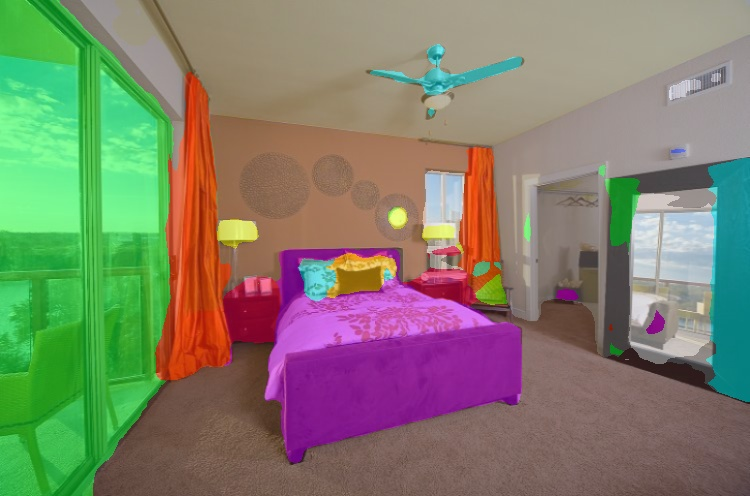
\includegraphics[width=1.5in, height=1.in]{Sea_b_00000129.jpg} 
	          
\includegraphics[width=1.5in, height=1.in]{Sea_b_00000200.jpg} 
	          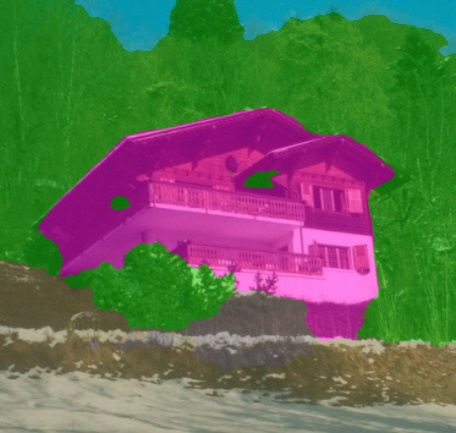
\includegraphics[width=1.5in, height=1.in]{Sea_b_00001239.jpg} 
	                                        }  \\                                      
	\centering
	\caption{Visualization of prediction results on ADE20K \textit{val} set.}
% 	\vspace{-0.2cm}
	\label{vis_results_2}
\end{figure*}

\section{Object detection}
To further demonstrate the generalization ability of our proposed SeaFormer++ backbone on other downstream tasks, we conduct object detection task on COCO dataset. 

We use RetinaNet~\cite{lin2017focal} (one-stage) as the detection framework and follow the standard settings to use SeaFormer++ as backbone to generate e feature pyramid at multiple scales. All models are trained  on train2017 split for 12 epochs (1×) from ImageNet pretrained weights.

From the table~\ref{table_coco_obj} We can observe that our SeaFormer++ achieves superior results on detection task which further demonstrates the strong generalization ability of our method.
\begin{table}[tb]
    \centering
    \small
    \begin{tabular}[b]{l | c |c |c }
    \hline

    \hline

    \hline
        Backbone & AP  & FLOPs    & Params\\

    \hline
        
    \hline
    \hline
    ShuffleNetv2~\cite{ma2018shufflenet} & 25.9  & 161G  & 10.4M   \\
    SeaFormer-T &  31.5        & 160G    & 10.9M        \\
    \textbf{SeaFormer-T++} &  \textbf{32.8}         & \textbf{160G}    & 11.0M        \\      \\
    \hline
          
    \hline
    \hline
    Mobile-Former151~\cite{chen2022mobile}   & 34.2   & 161G   & 14.4M\\
    MobileNetV3~\cite{howard2019searching} & 27.2  &162G   & 12.3M \\

    SeaFormer-S &  34.6           & 161G   & 13.3M         \\
    \textbf{SeaFormer-S++} &  \textbf{35.5}           & \textbf{161G}   & 13.4M         \\       \\
    \hline
        
    \hline
    \hline
    Mobile-Former214~\cite{chen2022mobile}     & 35.8  &\textbf{162G}    & 15.2M\\
    Mobile-Former294~\cite{chen2022mobile}     & 36.6   &164G   & 16.1M\\
    SeaFormer-B &  36.7      & 164G   &18.1M            \\
    \textbf{SeaFormer-B++} &  \textbf{37.4}      & 164G   &18.2M            \\
    \hline

    \hline
    \hline
    ResNet50~\cite{he2016deep} & 36.5  & 239G & 37.7M \\
    PVT-Tiny~\cite{wang2021pyramid} & 36.7  & 221G  & 23.0M  \\
    ConT-M~\cite{yan2021contnet} & 37.9  & 217G  & 27.0M   \\
    SeaFormer-L &  39.8      & 185G  &24.0M            \\
    \textbf{SeaFormer-L++} &  \textbf{40.2}       & \textbf{185G}    &24.1M            \\
         \hline

        \hline
        
        \hline
  \end{tabular}
\caption{Results on COCO object detecion.}
\label{table_coco_obj}
\end{table}

\begin{figure*}[tbp]
	\centering
	\subfloat[Ground Truth]{
               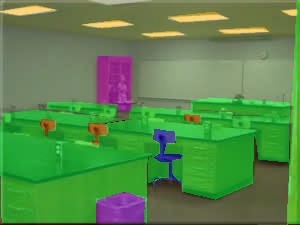
\includegraphics[width=1.5in, height=1.in]{gt_00000489.jpg} 
               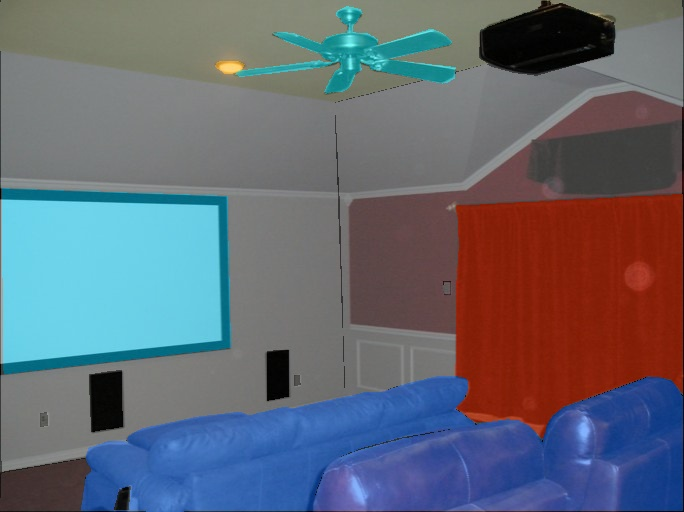
\includegraphics[width=1.5in, height=1.in]{gt_00000425.jpg} 
               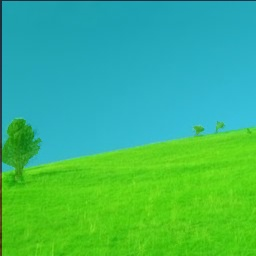
\includegraphics[width=1.5in, height=1.in]{gt_00000987.jpg} 
	                                        }\\

	\subfloat[SegFormer-B1~\cite{xie2021segformer}]{
	          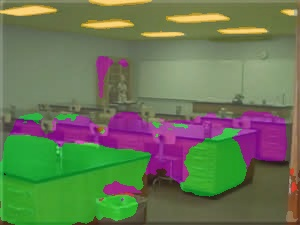
\includegraphics[width=1.5in, height=1.in]{Seg_b1_00000489.jpg} 
	          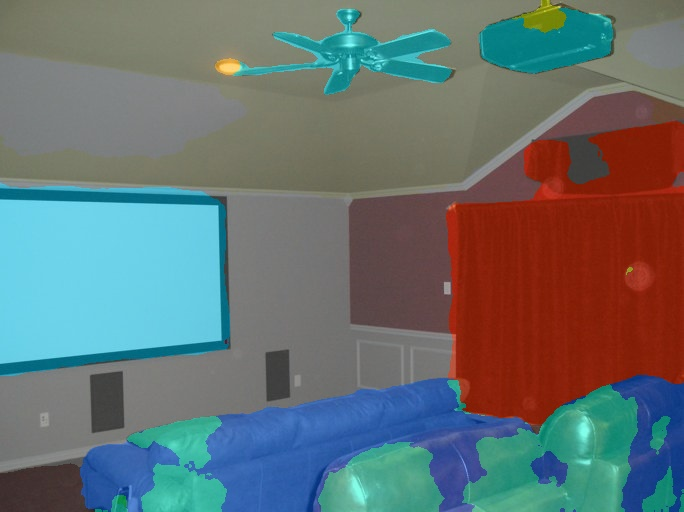
\includegraphics[width=1.5in, height=1.in]{Seg_b1_00000425.jpg} 
	          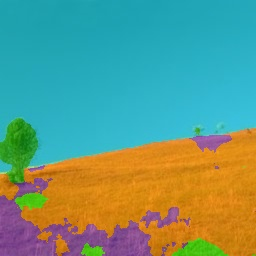
\includegraphics[width=1.5in, height=1.in]{Seg_b1_00000987.jpg} 
	                                        }\\
	\subfloat[SeaFormer-L (Ours)]{
	          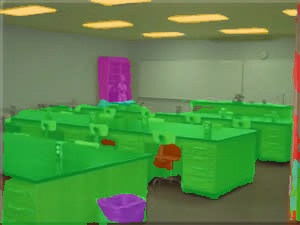
\includegraphics[width=1.5in, height=1.in]{Sea_l_00000489.jpg} 
	          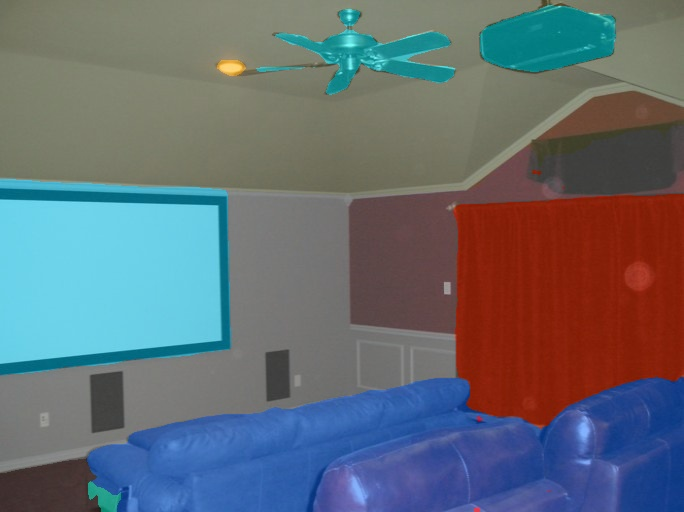
\includegraphics[width=1.5in, height=1.in]{Sea_l_00000425.jpg} 
	          
\includegraphics[width=1.5in, height=1.in]{Sea_l_00000987.jpg} 
	                                        }\\                                        
	\centering
	\caption{Visualization of prediction results on ADE20K \textit{val} set.}
% 	\vspace{-0.2cm}
	\label{vis_results}
\end{figure*}

\subsection{Latency statistics}
\begin{figure}
% \vspace{-5cm}
  \centering
   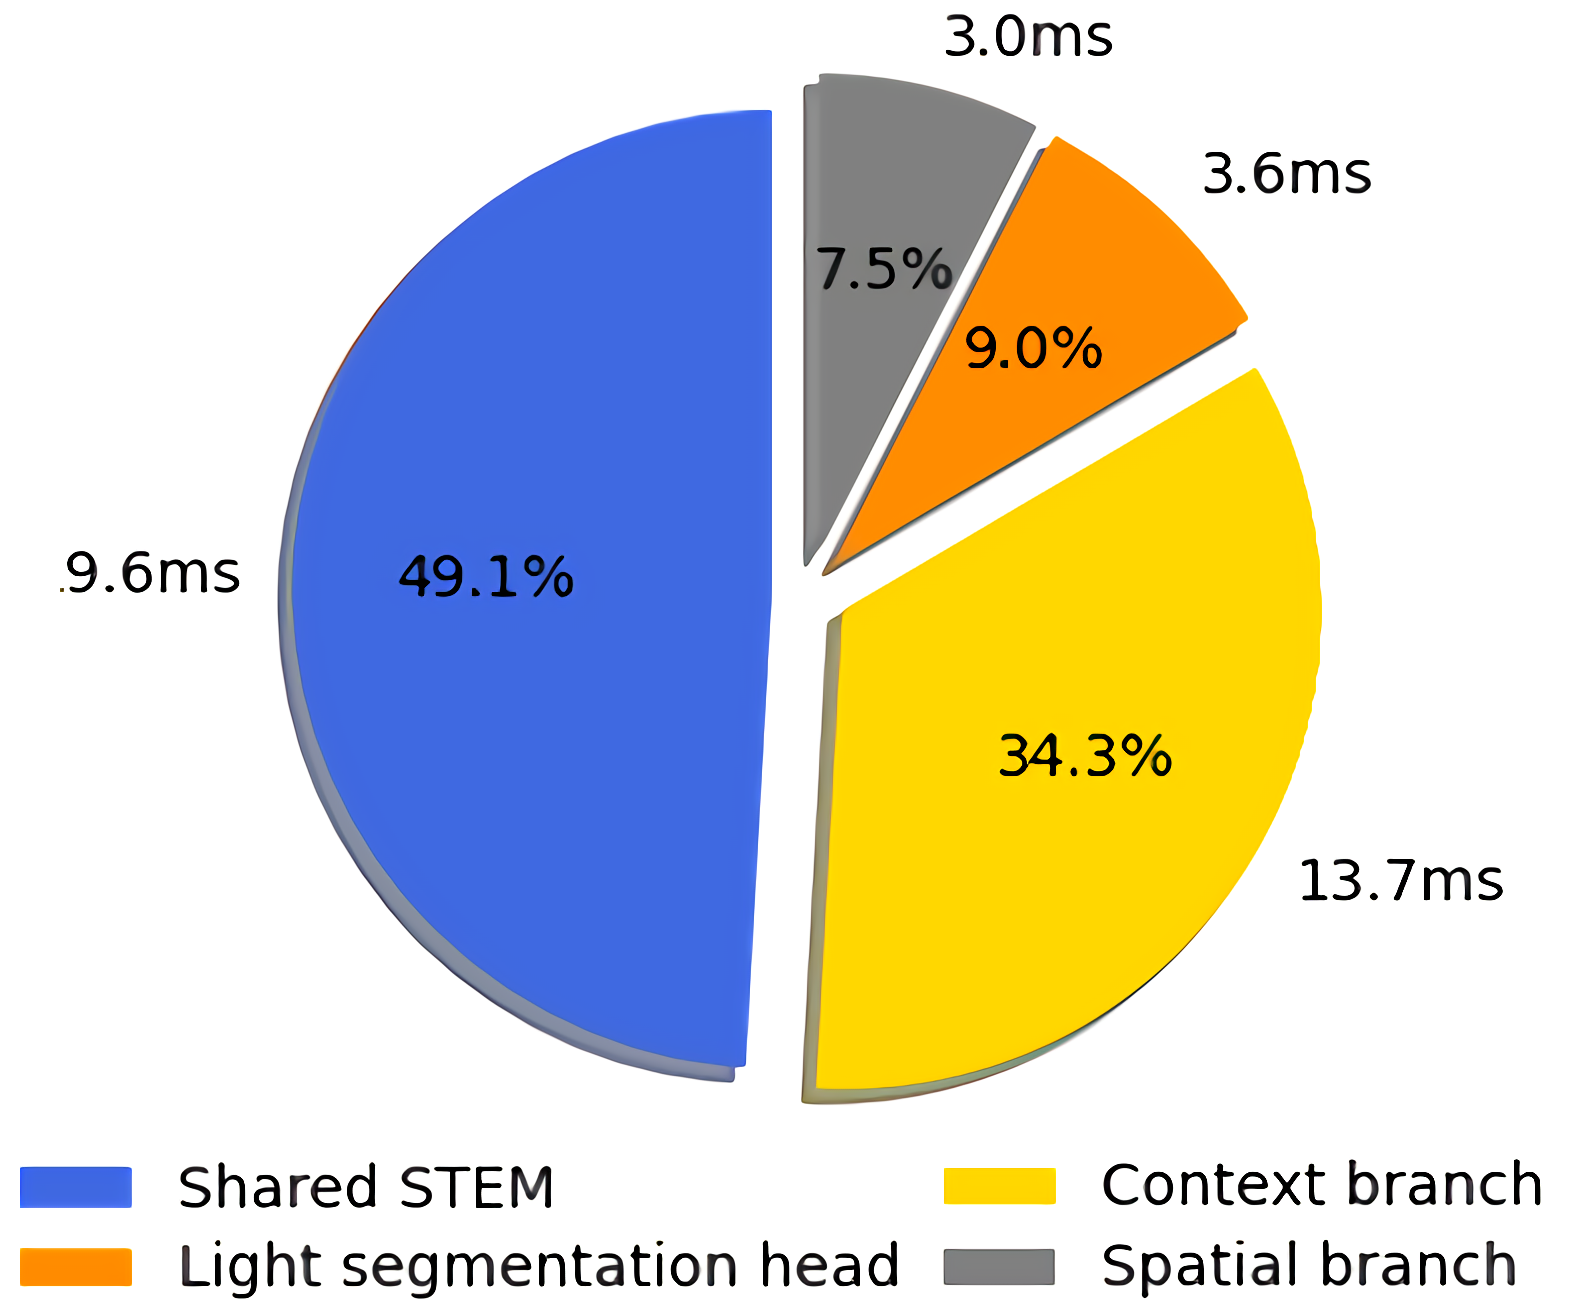
\includegraphics[scale=0.6]{latency_proportion.png}
  \caption{The inference latency of components.}
  \label{lat}
% \vspace{-0.1cm}
\end{figure}
We make the statistics of the latency of the proposed SeaFormer-Tiny, as shown in Figure~\ref{lat}, the shared STEM takes up about half of the latency of the whole network (49\%). 
The latency of the context branch is about a third of the total latency (34\%), 
whilst the actual latency of the spatial branch is relatively low (8\%) due to sharing early convolution layers with the context branch.
Our light segmentation head (8\%) also contributes to the success of building a light model.

\section{Performance under different precision of the models}
Following TopFormer, we measure the latency in the submission paper on a single Qualcomm Snapdragon 865, and only an ARM CPU core is used for speed testing. No other means of acceleration, e.g., GPU or quantification, is used. We provide a more comprehensive comparison to demonstrate the necessity of our proposed method. We test the latency under different precision of the models.
From the table~\ref{table_diff_precision}, it can be seen that whether it is full precision or half precision the performance of SeaFormer is better than that of TopFormer.
\begin{table}[tb]
    \centering

        \begin{tabular}{l|c|c|c}
        
        \hline
        
        \hline
        
        \hline
        Model  &  mIoU & FP32 & FP16 \\
        \hline
        
        \hline
        \hline
        TopFormer-T	&34.6	&43ms	&23ms \\
        \textbf{SeaFormer-T}	&\textbf{35.8}	&\textbf{40ms}	&\textbf{22ms}\\
        TopFormer-S	&37.0	&74ms	&41ms\\
        \textbf{SeaFormer-S}	&\textbf{39.4}	&\textbf{67ms}	&\textbf{36ms}\\
        TopFormer-B	&39.2	&110ms	&60ms\\
        \textbf{SeaFormer-B}	&\textbf{41.0}	&\textbf{106ms}	&\textbf{56ms}\\
        SeaFormer-L	&43.7	&367ms	&186ms\\

        \hline
        
        \hline
        
        \hline
    \end{tabular}
    \caption{Performance comparison on ADE20K \textit{val} set under different precision.}
        \label{table_diff_precision}
\end{table}

\section{Visualization}

\subsection{Attention heatmap}
To demonstrate the effectiveness of detail enhancement in our squeeze-enhanced Axial attention (SEA attention),
we ablate our model by removing the detail enhancement. 
We visualize the attention heatmaps of the two models in Figure~\ref{heatmap_vis}.
Without detail enhancement, attention heatmaps from solely SA attention appears to be axial strips while our proposed SEA attention is able to activate the semantic local region accurately, which is particularly significant in the dense prediction task.

\subsection{Prediction results}
We show the qualitative results and compare with the alternatives on the ADE20K validation set from two different perspectives. 
First we compare with a mobile-friendly rival TopFormer~\cite{zhang2022topformer} with similar FLOPs and latency in Figure~\ref{vis_results_2}. 
Besides, we compare with the Transformer-based counterpart SegFormer-B1~\cite{xie2021segformer} in Figure~\ref{vis_results}.
In particular, our SeaFormer-L has lower computation cost than the SegFormer-B1.
As shown in both figures, we demonstrate better segmentation results than both the mobile counterpart and Transformer-based approach.

\section{Multi-resolution distillation based on feature up-sampling}
\subsection{Experimental setup} We perform multi-resolution distillation experiments over ADE20K~\cite{zhou2017scene}. The mean of intersection over union (mIoU) is set as the evaluation metric. 
We convert full-precision models to TNN~\cite{contributors2020tnn} and measure latency on an ARM-based device with a single Qualcomm Snapdragon 865 processor.
We set ADE20K fine-tuned network with original resolution input in section~\ref{Exp} as the teacher model and ImageNet-1K~\cite{deng2009imagenet} pretrained network as the backbone of the student model.
The input resolution of the student model is halved by average pooling.

The standard BatchNorm~\cite{ioffe2015batch} layer is replaced by synchronized BatchNorm.
The implementation of multi-resolution distillation is based on public codebase \texttt{mmsegmentation}~\cite{contributors2020mmsegmentation}.
We follow the batch size, training iteration scheduler and data augmentation strategy of TopFormer~\cite{zhang2022topformer} and section~\ref{Exp} for a fair comparison.
The initial learning rate is 0.0005 for batch size 32 or 0.00025 for batch size 16. The weight decay is 0.01. 
A “poly” learning rate scheduled with factor 1.0 is adopted.
During inference, we set the same resize and crop rules as TopFormer to ensure fairness.

\subsection{Comparison with state of the art}
Table~\ref{ade20k_table} shows the results of SeaFormer++ (KD) and previous efficient backbones on ADE20K \textit{val} set. 
The comparison covers Params, FLOPs, Latency and mIoU. 
As shown in Table~\ref{ade20k_table}, SeaFormer++ (KD) outperforms these efficient approaches with extremely less FLOPs and lower latency. 

\subsection{Ablation studie}
This study conducts ablation experiments to evaluate various upsampling modules and loss function configurations for reducing computational demands and maintaining performance in visual tasks. It aims to identify efficient upsampling strategies and optimal loss combinations that preserve model accuracy. Experiments were standardized on the ADE20K validation set to ensure fair comparison and result reliability. The research compares the efficacy of techniques like bilinear interpolation, lightweight MobileNetV2-based upsampling, and standard convolutional upsampling, assessed by mean Intersection over Union (mIoU) and computational impact. Adjusting loss functions, including classification loss, cross-model classification loss, feature similarity loss, and output similarity loss, further analyzes their role in knowledge distillation effectiveness. These experiments offer insights into balancing efficiency and performance in model design, providing a methodology for exploring model enhancements under computational constraints and guiding optimal configurations for accurate visual recognition in practical applications.

\paragraph{Impact of upsample module design}
We compare three different upsampling strategies: direct bilinear interpolation, MobileNetV2-based upsample module, and standard convolution-based upsample module.
\begin{table}[ht]
\centering
\begin{tabular}{lcccc}
\hline

\hline

\hline
Upsampling Module & \#Params & FLOPs &  mIoU & Latency \\
\hline
Direct Interpolation & 1.7M & 0.3G & 33.7 & 20ms\\
MobileNetV2-based upsample module & 2.3M & 0.3G & 35.5 & 22ms \\
tandard convolution-based upsample module & 2.7M & 0.4G & 35.7 & 30ms\\
\hline

\hline

\hline
\end{tabular}
\caption{Ablation study results of the upsampling modules.}
\label{tab:upsampling_ablation}
\end{table}
In this section, the effects of three upsampling strategies on model performance were compared. The direct interpolation approach, while requiring the least parameters (1.7M) and computational effort (0.3G FLOPs), resulted in the lowest mIoU (33.7\%) and the least latency (20ms), suggesting limited complexity handling. The MobileNetV2-based lightweight upsampling improved mIoU to 35.5\% with a slight latency increase to 22ms, offering a balanced performance enhancement. The standard convolution-based module, although yielding the highest mIoU (35.7\%), did so at the cost of increased parameters (2.7M), computation (0.4G FLOPs), and latency (30ms). These findings highlight a trade-off between performance and speed in upsampling choices, with the MobileNetV2-based module providing an optimal balance for dense prediction tasks on resource-constrained devices.

\paragraph{Impact of loss function}
We incrementally add four loss function components—classification loss, output similarity loss, feature similarity loss, and cross-model classification loss—to assess their contribution to model performance.
\begin{table}[ht]
\centering
\begin{tabular}{ccccc}
\hline

\hline

\hline
Cls loss & Out loss & Feat loss & Cross loss &  mIoU \\
\hline
\checkmark & & & &  32.5\\
\checkmark &\checkmark & & &  33.7\\
\checkmark &\checkmark &\checkmark & &  34.7\\
\checkmark &\checkmark &\checkmark &\checkmark &  35.5\\
\hline

\hline

\hline
\end{tabular}
\caption{Ablation study results of loss function design.}
\label{tab:loss_ablation}
\end{table}
Through ablation studies, this experiment evaluates the performance impact of different loss functions in semantic segmentation, involving "classification loss," "output similarity loss," "feature similarity loss," and "cross-model classification loss," with mIoU as the evaluation metric. Starting from a baseline mIoU of 32.5 with just classification loss, performance sequentially improves with the addition of output and feature similarity losses, highlighting the benefits of aligning student and teacher model outputs and features for accuracy. The highest mIoU of 35.5 is achieved with the inclusion of cross-model classification loss, emphasizing the effectiveness of combining various constraints on the student model. The results underscore the individual and collective contributions of each loss function to semantic segmentation tasks, particularly the significance of model alignment for substantial performance gains, and the synergistic enhancement of model performance through integrated loss function design.




